\chapter{Concetti introduttivi}

\section{L'attività di testing}

\subsection{Introduzione}

Poiché l'argomento principale di questa trattazione consiste nell'analisi di alcune strategie di test applicate al caso particolare delle applicazioni web, è opportuno introdurre l'argomento descrivendo alcuni concetti teorici basilari, che permettono di comprendere meglio il contesto in cui andranno ad operare gli strumenti analizzati.

Le tipologie di testing tradizionalmente individuate nell'ingegneria del software si suddividono in base al livello architetturale interessato dalle verifiche.
Il software infatti può essere modellizzato attraverso una serie di componenti che interagiscono tra di loro. A seconda del caso, ci si può concentrare sul funzionamento dei vari moduli in isolamento, oppure sul comportamento globale del sistema, una volta che i moduli vengono integrati e interagiscono tra loro, oppure ancora sull'integrazione del software con altri componenti esterni, generalmente non controllabili direttamente dal sistema sviluppato.

Un altro dei principali criterio di classificazione si basa sul ruolo svolto dalle figure che definiscono ed eseguono le verifiche. Nei casi più comuni, esse vengono definite da uno o più gruppi di programmatori interni all'organizzazione che realizza il software e il loro utilizzo rimane pertanto confinato in questo ambito.

In altri casi invece è la figura del committente che può avere interesse a stabilire un'insieme di verifiche sul prodotto richiesto, per assicurarsi che esso raggiunga un certo grado di affidabilità e che rispetti le funzionalità promesse a livello contrattuale. Questi test sono volutamente indipendenti da quelli interni e spesso sono definiti da personale che possiede competenze nel campo di utilizzo del software ma non nell'ambito delle tecnologie adoperate. 

\subsection{Unit testing}
Nello unit testing il comportamento dei vari moduli che compongono il software viene verificato in isolamento. Estrapolando la logica di ogni componente dal contesto in cui essa viene utilizzata, risulta più semplice verificarne il corretto comportamento, siccome si evita che alcuni possibili errori vengano mascherati dalle interazioni con il resto del sistema. 

Inoltre i difetti possono essere rivelati e corretti in maniera più rapida, poiché si riduce la complessità del problema attraverso il classico paradigma \emph{divide et impera} e di conseguenza l'area in cui individuare la causa del problema sarà maggiormente circoscritta.

Affinché questa tecnica sia applicabile, è fondamentale progettare il software in maniera modulare, adottando le regole tipiche della programmazione ad oggetti. In aggiunta, è necessario ridurre al minimo i vincoli di dipendenza tra i componenti, in modo che ognuno possa essere trattato come una entità logica a sé stante, con responsabilità ben delineate e con un funzionamento verificabile quindi in maniera indipendente.

Solitamente, all'interno del paradigma della programmazione ad oggetti l'unità elementare interessata dallo unit testing è la classe. Si ricercano potenziali problemi nel funzionamento atteso fornendo in ingresso ai metodi pubblici
svariati insiemi di dati, che si ritiene possano provocare comportamenti critici del codice. 

Nello specifico, spesso si utilizzano insiemi di input, chiamati \emph{boundary values}, che sollecitano il funzionamento dell'unità ai limiti dei valori normalmente attesi in ingresso. 
Normalmente infatti chi sviluppa il codice sotto esame si concentra sul caso tipico di utilizzo e tralascia con maggiore probabilità i casi poco frequenti o inaspettati. Siccome successivamente i moduli saranno integrati, è opportuno perciò assicurarsi che essi reagiscano ragionevolmente anche alle situazioni impreviste, in modo da individuare più agevolmente i problemi che si verificheranno negli stadi successivi di sviluppo e di testing.

\subsection{Integration testing}

Il passo successivo allo unit testing è l'integration testing. A questo livello, la verifica si concentra sull'interazione tra i componenti utilizzati nel software. Sebbene essi siano stati testati in precedenza attraverso lo unit testing, non è garantito che il loro comportamento sia quello atteso una volta che questi si trovano ad operare insieme, poiché potrebbero sorgere nuovi problemi nei punti di interconnessione.

Se lo unit testing è stato effettuato in maniera adeguata, lo sviluppatore avrà a questo punto sufficiente confidenza nel fatto che i difetti saranno concentrati principalmente nel modo in cui i moduli sono utilizzati insieme.

Affinché si possano trarre i maggiori benefici da questo approccio, è importante poter effettuare i test di integrazione in maniera incrementale, aggiungendo cioè uno alla volta i componenti da integrare. Per fare ciò, spesso si utilizzano delle versioni simulate di alcuni componenti, dette \emph{stub}, il cui comportamento è prestabilito in maniera artificiale dal programmatore. Gli stub permettono quindi di simulare il comportamento dei componenti non ancora integrati o addirittura non ancora sviluppati e consentono di concentrare i test sull'integrazione di pochi componenti reali alla volta, riducendo i gradi di libertà del sistema.

\subsection{Functional testing}

Nei livelli visti fino ad ora, i criteri di validazione per i test sono definiti in base a scelte funzionali e di design dettate dai progettisti e dagli sviluppatori, cioè da quelle figure che si occupano della realizzazione del software. 
Se ci si limita a questo livello, nulla garantisce che il software, una volta ultimato, rispettassi i requisiti e le specifiche dettati da chi ha commissionato il lavoro che si sta svolgendo. Pertanto, si correre il rischio di sviluppare un progetto
che visto dall'interno risulta funzionare in maniera corretta (nei casi sotto esame), ma che dall'esterno non dimostra effettiva utilità a vantaggio dell'utilizzatore finale.

Attraverso il functional testing si cerca quindi di assicurare la conformità del software realizzato rispetto ai requisiti di partenza. 

Il livello di astrazione a cui questo tipo di test opera è il più elevato rispetto alle metodologie descritte in precedenza, poiché nella definizione delle verifiche si perde il dettaglio su come il codice sia strutturato. Ciò che interessa verificare è proprio la \emph{funzionalità} fornita dal progetto sotto esame.

\subsection{Acceptance testing}

Secondo \cite{KanerFalk}, con il termine \emph{acceptance testing} si indicano generalmente le verifiche che il cliente finale (o chi ha commissionato il software) esegue per assicurarsi che il prodotto si comporti secondo le proprie esigenze, e che quindi il suo utilizzo produca un certo tipo di valore aggiunto.

Normalmente questo tipo di validazione viene quindi svolto da persone esterne all'organizzazione che sta sviluppando il progetto, o comunque in stretta collaborazione tra il committente e gli sviluppatori. 

Questa tipologia di test si occupa di evidenziare in maniera rapida i principali difetti riscontrabili nel software. Non vengono verificati tutti i dettagli presenti, ma solamente le funzionalità principali, in modo da poter stabilire subito se il software rispetta i requisiti di base attesi.

Poiché i test di accettazione devono essere eseguiti in corrispondenza di ogni nuova versione rilasciata, è importante poter automatizzare questo processo per diverse ragioni. Innanzitutto la definizione dei test è un'attività che può richiede un'importante quantità di tempo e che deve essere svolta frequentemente, con relativo dispendio di risorse economiche. A causa di questo fattore spesso si tende a trascurare questa fase, che però svolge un ruolo fondamentale per assicurare un grado di qualità minimo nel prodotto acquistato. In aggiunta, eseguire manualmente le operazioni principali all'interno del software per definire i test è un'attività noiosa e ripetitiva, e spesso per questo motivo si può essere tentati di evitare alcuni passaggi, che potrebbero però rivelarsi importanti ai fini delle verifiche.

Se usati in maniera corretta, I test di accettazione svolti dal committente possono anche rappresentare un utile mezzo di comunicazione con il team di sviluppo. Attraverso questi test infatti il committente può identificare in maniera precisa e riproducibile i difetti riscontrati e comunicarli agli sviluppatori in modo che possano essere corretti il prima possibile. Inoltre, il committente può stabilire attraverso i test quali siano le funzionalità principali da implementare in maniera prioritaria, permettendo al team di programmatori di concentrarsi su di esse.

%\section{Test Driven Development}

%\section{Behavior Driven Development}

\section{Il testing delle interfacce grafiche}

\subsection{Introduzione}

L'attività che riguarda la verifica e la validazione di interfacce grafiche richiede tecniche e strategie particolari, sebbene i criteri fondamentali ed i processi di implementazione siano poi gli stessi che sono validi per il testing convenzionale ~\cite{memonGuiTesting}.

Gli aspetti peculiari di tale attività hanno richiesto lo sviluppo di strumenti e di framework pensati apposta per questo compito. Al giorno d'oggi la stragrande maggioranza delle applicazioni utilizza un'interfaccia grafica per comunicare con l'utente, pertanto da diversi decenni il testing delle interfacce è divenuto una pratica consolidata nell'ingegneria del software.

In riferimento alla panoramica descritta nel capitolo precedente, questa attività interessa praticamente tutti i livelli descritti: nello sviluppare un framework per la creazione e la gestione di interfacce grafiche sono effettuati test ad ognuno dei livelli indicati finora.

Tuttavia, se come accade poi nella pratica viene utilizzato un sistema di librerie già precostruito per implementare l'interfaccia grafica dell'applicazione, allora diventa poco sensato effettuare una serie di test per ogni livello, in quanto ci si fida della qualità del codice utilizzato e creato apposta per lo scopo.

Sotto questa ipotesi, il testing di interfacce grafiche si colloca ad un livello di astrazione e di generalità molto elevato. Può essere classificato infatti nella categoria dei test di integrazione, poiché per verificare il corretto comportamento dell'interfaccia è necessario stimolare contemporaneamente un elevato numero di componenti del sistema. 

Inoltre, le sequenze di operazioni che si vanno a riprodurre durante i controlli tendono ad avvicinarsi a quelle che potrebbe eseguire direttamente l'utente finale, durante il normale utilizzo del software in questione. Ecco quindi che, sotto un certo punto di vista, questa verifica si può considerare simile ad un test di accettazione, siccome i requisiti sotto esame saranno verosimilmente simili a quelli stabiliti dalle parti che hanno commissionato la realizzazione, visto l'elevato livello di astrazione a cui si opera.

Si può inoltre osservare che le verifiche eseguite durante questa tipologia di test sollecitano indirettamente anche livelli architetturali meno astratti rispetto a quelli indicati fino ad adesso. 

Infatti, affinché i test risultino efficaci, è necessaria la partecipazione di tutti gli strati logici che compongono l'applicazione, poiché inevitabilmente l'interfaccia è collocata al di sopra di essi e con essi interagisce pesantemente. In particolare, saranno verificate indirettamente alcune delle cosiddette \emph{business rule}, ossia quella parte di logica nel software che implementa le operazioni da effettuare sui dati ed i vincoli su di esse nel rispetto dei requisiti dettati dal committente \cite{agileRequirements}.

In merito a quest'ultima osservazione  è bene notare che, nonostante la sua potenziale ambivalenza, il testing che interessa l'interfaccia grafica non deve sostituire la serie di verifiche sul software ai livelli inferiori nella panoramica vista fino ad ora: è fondamentale che ogni strato venga verificato dalla tipologia di test adeguata (unit test per i moduli, integration test per il sistema, eccetera). In \cite{microsoft} la corretta sovrapposizione dei vari livelli di test viene schematizzata tramite il diagramma a piramide mostrato in figura ~\ref{fig:testPyramid}. In questo schema, l'ampiezza dei gradini indica inoltre che è opportuno assegnare eseguire un maggior numero di test in corrispondenza dei livelli più bassi, poiché in essi risiedono le fondamenta su cui si basa il resto dell'applicazione.

\begin{figure}[htbp]
\begin{center}
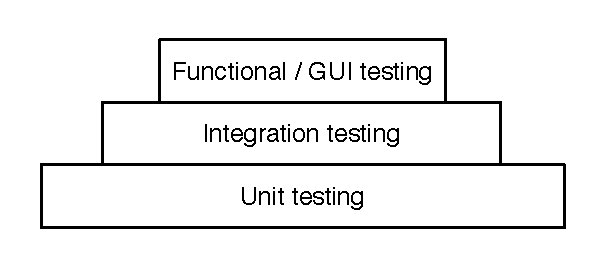
\includegraphics[width=\textwidth]{images/test_pyramid.eps}
\caption{Sovrapposizione dei livelli di test}
\label{fig:testPyramid}
\end{center}
\end{figure}

\subsection{Problematiche}

In base a quanto visto fino ad ora, è logico aspettarsi che la verifica di interfacce grafiche sia un'attività complessa, dato l'ampio spettro in cui essa agisce.
Infatti, durante questa fase si incontrano diverse problematiche, che pongono spesso severi limiti entro i quali ci si può muovere. Persino la strategia adottata per definire gli scenari da verificare assume una notevole importanza sull'efficacia di queste verifiche, poiché la complessità dell'interfaccia richiede di selezionare solo un ridotto sottoinsieme dei test che è possibile eseguire, come mostrato in \cite{guiTestGeneration}.

Nei paragrafi seguenti vengono presentati gli aspetti critici che si devono affrontare durante il test di interfacce grafiche.

\subsubsection{Complessità intrinseca del sistema}
Siccome un'interfaccia grafica è pensata principalmente per facilitare e rendere più naturale l'interazione dell'utente con il software, essa deve fornire funzionalità di alto livello, che si traducono in una varietà di controlli e di elementi molto variegata. Normalmente esistono molti percorsi possibili attraverso i quali l'utente può eseguire la stessa operazione, ed il numero di eventi che possono essere generati (pressione di tasti, click del mouse, etc.) è potenzialmente illimitato.

Questi fattori originano poi interdipendenze e problemi di sincronizzazione tra i componenti dell'interfaccia, poiché i dati inseriti come input possono essere mostrati contemporaneamente in aree differenti e con una diversa modalità di rappresentazione. Spesso i dati sono modificabili direttamente nelle aree di visualizzazione ed è necessario un costante aggiornamento per allineare i dati in memoria con quelli mostrati all'utente.

Inoltre, è ragionevole pensare che più un'interfaccia risulta essere utile all'utente, più essa richiede un grado di complessità maggiore, per permettere di eseguire operazioni complesse. Come diretta conseguenza,  aumentano le difficoltà nell'acquisizione e nella gestione dei test. Difficilmente infatti, in situazioni reali sono sufficienti poche finestre e pochi elementi per utilizzare in modo flessibile applicazioni professionali. 

Infine, data la complessità del codice, è fondamentale che il framework utilizzato per generare l'interfaccia grafica sia strutturato secondo schemi di design che permettano con relativa facilità di effettuare le verifiche necessarie sui componenti grafici. Da questo punto di vista, la scelta iniziale sulle tecnologie da utilizzare per realizzare l'applicazione può assumere un peso notevole nell'ottica dei test.

\subsubsection{Registrazione e riproduzione dei dati in ingresso}

Come scritto in precedenza, a differenza di un programma a linea di comando, un'interfaccia grafica può accettare input dall'utente attraverso svariati modi e soprattutto con tempistiche non prevedibili a priori. Questa situazione rende particolarmente difficile sia la riproduzione che l'acquisizione dei dati inseriti dall'utente per riprodurre il test in maniera automatica. 

Gli eventi come il click del mouse o la pressione di un tasto sono generalmente gestiti prima dal sistema operativo, che provvede a notificarli all'applicazione. Il linguaggio e le librerie utilizzate devono fornire agli sviluppatori la possibilità di intercettare questi eventi durante il test e di simularli in maniera programmatica, altrimenti risulta impossibile tentare di eseguire la sequenza di operazioni sull'interfaccia che sono oggetto di verifica.

Se l'applicazione su cui andranno effettuati i test viene sviluppata da zero, si potranno scegliere soluzioni che facilitino l'esecuzione di verifiche sull'interfaccia, mentre se ci si trova ad eseguire in un secondo momento dei test su un'applicazione già esistente l'esecuzione di una test suite potrebbe essere problematica.

\subsubsection{Regression test}

I test effettuati su interfacce grafiche sono tendenzialmente molto sensibili ai cambiamenti di aspetto che intercorrono durante l'evoluzione dell'applicazione. Spesso infatti può bastare uno spostamento di posizione di un pulsante o di un campo di testo affinché un test fallisca, senza che però si verifichino problemi effettivi nell'uso dell'interfaccia. 

Ciò accade perché durante la scrittura del test si deve prendere come punto di partenza la collocazione dei vari elementi nell'interfaccia grafica, ma quest'ultima non rispecchia necessariamente la funzionalità sottostante. Si rischia quindi di preparare una serie di verifiche troppo dettagliate, che diventano pressoché inutilizzabili poiché richiedono un eccessivo lavoro di riscrittura a seguito di piccole variazioni apportate all'organizzazione grafica dell'interfaccia.

Un altro aspetto che rende questi test particolarmente fragili risiede nella necessità di tradurre in diverse lingue l'interfaccia di un'applicazione. Si supponga ad esempio che attraverso un semplice test si controllino i messaggi mostrati all'utente in seguito ad una certa operazione: se non si tiene in conto questo fattore, la verifica automatica potrebbe fallire solamente perché il messaggio può essere mostrato in una lingua differente da quella ipotizzata nel test.

In aggiunta, il livello di specificità necessario per rendere effettiva una verifica su di una interfaccia non può essere definito a priori. A seconda dei casi, potrebbe essere richiesto di controllare l'esatta posizione e dimensioni di un elemento nella finestra dell'applicazione sotto esame, mentre in altri ambiti può essere sufficiente verificare la risposta dell'interfaccia in seguito ad un evento generato dall'utente su quell'elemento, indipendentemente dalla sua collocazione o dal suo aspetto.
Gli strumenti attraverso i quali sono definiti i test devono essere in grado di operare su livelli differenti e spesso ci si trova a dover usare strumenti differenti per eseguire differenti tipi di test su scenari d'uso equivalenti.

In alcuni casi l'uso di questi strumenti per automatizzare i test può non trovare una giustificazione valida in termini di tempo e di costi. Se lo sviluppo dell'interfaccia avviene attraverso l'uso di prototipi o segue un approccio dove le modifiche sono molto frequenti, i costi derivati dalla realizzazione e dall'aggiornamento costante dei regression test potrebbero superare i benefici ottenuti dall'automazione (\cite{gerrardGUI}). 

\subsubsection{Definizione di metriche}

Per le attività di verifica più tradizionali sono definite svariate metriche, le quali permettono di avere una misurazione oggettiva su alcuni criteri importanti per definire degli standard di qualità sul codice prodotto. Ad esempio, una delle metriche più diffuse consiste nel conteggio delle linee di codice all'interno di un software che sono effettivamente eseguite durante i test. 

Attraverso questa misura è possibile avere in maniera semplice un'indicazione sulla percentuale di codice scritto che è stato sottoposto a verifica. In base ai propri criteri, si può quindi stabilire una soglia che definisce quando il numero di test prodotti può essere considerato sufficiente. Negli anni sono poi state raccolte numerose statistiche in base alla distribuzione dei difetti all'interno dei vari moduli, che forniscono indicazioni utili per concentrare efficacemente gli sforzi di verifica sulle aree più interessate da potenziali difetti.

Per quanto riguarda il caso particolare delle interfacce grafiche, è molto più difficile stabilire metriche e criteri obiettivi che guidino in questo senso la scrittura dei test. Data la potenziale complessità descritta in precedenza che si deve affrontare, può risultare difficile anche solo stabilire in che percentuale il funzionamento dell'interfaccia grafica sia stato verificato.

\subsection{Il testing delle interfacce nelle applicazioni web}

Rispetto al caso delle applicazioni desktop, il testing delle interfacce utilizzate nelle applicazioni web presenta le stesse problematiche di base descritte in precedenza, ma allo stesso tempo richiede un'analisi a parte, in quanto sussistono profonde differenze dal punto di vista delle tecnologie usate, del livello di interazione con l'utente, e soprattutto nelle metodologie di implementazione.

Inoltre, le due tipologie di applicazioni vengono eseguite in ambienti completamente differenti (il sistema operativo ed il browser), e si trovano quindi a dover sottostare a vincoli di realizzazione molto differenti tra loro.

Se le applicazioni desktop sono orami una realtà consolidata da parecchi decenni, le applicazioni web hanno iniziato a dimostrarsi realmente come potenziali rivali solo negli ultimi anni. A titolo di campione, si prenda in esame la seguente tabella \footnote{\url{http://www.crunchbase.com}}, che indica l'anno in cui i maggiori competitor hanno reso disponibili pubblicamente le applicazioni web più utilizzate ad oggi.

\begin{table}[htdp]
\caption{Anno di lancio delle maggiori applicazioni web}
\begin{center}
\begin{tabular}{l l l}
	\hline
	\textbf{Nome applicazione} & \textbf{Organizzazione} & \textbf{Mese e anno di lancio} \\
	\hline
	Basecamp & 37signals & febbraio 2004\\ 
	\hline
	Flickr & Yahoo! & febbraio 2004\\ 
	\hline
	Twitter & Obvious Corp & luglio 2006\\
	\hline
	GMail & Google & febbraio 2007\\
	\hline
	GoogleReader & Google & settembre 2007\\
	\hline
	GoogleWave & Google & maggio 2009\\
	\hline
	GooleMaps & Google & maggio 2008\\
	\hline
	Facebook & Facebook, Inc. & febbraio 2004\\
	\hline
\end{tabular}
\end{center}
\label{default}
\end{table}

Viene proposta di seguito una breve analisi delle peculiarità riscontrabili nelle applicazioni web rispetto a quelle desktop, in modo da rendere più chiare alcune scelte prese nel proseguo della trattazione.

\subsection{Differenze tecnologiche}

Per definizione un'applicazione web viene utilizzata attraverso un browser. Di conseguenza, la scelta delle tecnologie da utilizzare per l'implementazione dell'interfaccia è strettamente limitata a quelle messe a disposizione dal browser. 
Ad oggi, le tecnologie maggiormente diffuse sono le seguenti:

\begin{description}
\item[HTML:] il linguaggio di markup per la definizione degli elementi semantici e strutturali che compongono la pagina web
\item[CSS:] un sistema di regole che definiscono la presentazione grafica e la disposizione degli elementi definiti tramite l'HTML
\item[Javascript:]  un linguaggio di scripting nato per essere interpretato dal browser, che mette a disposizione un'interfaccia per accedere al modello gerarchico della pagina (DOM) e ad alcune funzionalità del browser
\item[Flash:] una piattaforma multimediale proprietaria per aggiungere animazioni, video, e nuove possibilità di interazione alle pagine web. I file flash, scritti tramite il linguaggio ActionScript, vengono inclusi nella pagina come risorse esterne. Attualmente, l'uso di questa tecnologia è in declino,  soprattutto ora che i maggiori browser iniziano ad implementare le specifiche HTML5.
\end{description}

Queste tecnologie hanno scopi distinti, e costituiscono le componenti fondamentali per realizzare l'interfaccia grafica di un'applicazione web. Per implementare quest'ultima è quindi necessario utilizzare contemporaneamente tecnologie molto eterogenee tra di loro: ciò rende più difficoltosa la fase di testing poiché i metodi da utilizzare devono tener conto dell'azione di molteplici fattori. 

Ognuna di queste componenti tecnologiche può essere verificata in maniera indipendente, ad esempio effettuando la validazione automatica dell'HTML prodotto secondo la DTD specificata tramite il servizio online del W3C \footnote{W3C Validator \url{http://validator.w3.org}} , oppure eseguendo unit test sul codice javascript, ma la difficoltà principale risiede nel mettere alla prova la corretta interazione tra queste differenti tecnologie. 

Le interfacce grafiche per applicativi desktop sono invece solitamente realizzate attraverso il linguaggio principale di sviluppo utilizzato nel progetto. Questo fa sì che le tecniche di testing siano generalmente più omogenee e che non vi sia una marcata differenza concettuale tra il testing applicato ai vari livelli strutturali del software, cosa che invece è inevitabile per le applicazioni web.

Un'altra notevole differenza risiede nel fatto che le interfacce desktop sono implementante attraverso i paradigmi classici della programmazione ad oggetti. In tutti i framework più utilizzati, i vari \emph{widget} sono incapsulati in classi che seguono i paradigmi di design tipici dell'ingegneria del software. Nella fase di definizione e scrittura dei test è possibile sfruttare questa organizzazione razionale dei moduli sotto esame, migliorando notevolmente la flessibilità nella definizione delle verifiche, e rendendone la gestione più semplice. 

Poiché si utilizza un'organizzazione ad oggetti, i componenti dell'interfaccia grafica esporranno infatti delle interfacce pubbliche ben definite, secondo le buone norme della programmazione ad oggetti, che renderanno più evidenti i punti di aggancio per il codice che si occuperà di effettuare le verifiche. Inoltre, gli stessi eventi generabili dall'utente saranno tendenzialmente implementati tramite oggetti e gli errori o gli stati di inconsistenza modellati tramite eccezioni, rendendone la verifica e la riproduzione più agevole in fase di testing.

Di contro, nella stragrande maggioranza dei casi un'interfaccia realizzata tramite HTML, CSS e Javascript non possiede un'architettura logica ben definita, e ciò è imputabile a diversi fattori. 
In primo luogo alla scarsa omogeneità tra le tecnologie utilizzate, che poco si prestano per la loro natura ad essere organizzate secondo criteri funzionali: basti pensare che due di esse non sono neanche linguaggi di programmazione, ma semplici regole di formattazione o di markup. 

In secondo luogo, solo negli ultimi si è iniziato a diffondere interesse nella ricerca di nuovi strumenti per colmare le distanze tra le metodologie di sviluppo delle cosiddette \emph{rich web application} rispetto alle classiche applicazioni desktop. Sono nati così negli ultimi anni diversi progetti che tentando di trasferire al web l'esperienza accumulata nello sviluppo di interfacce grafiche tradizionali. A titolo di esempio si possono citare i seguenti progetti open-source:

\begin{description}
\item[Cappuccino]  \footnote{\url{http://cappuccino.org}}, un framework open source per facilitare lo sviluppo di applicazioni web simili ai software desktop, astraendo la complessità di utilizzare HTML e CSS per il layout grafico. Il framework utilizza un linguaggio chiamato Objective-J (compilato poi in javascript), che si ispira fortemente all'Objective-C utilizzato nel framework Cocoa per lo sviluppo di applicazioni su sistema operativo Apple OSX. Nel progetto è anche incluso un framework di testing con il nome di OjTest e sono presenti alcuni strumenti sperimentali per automatizzare il testing dell'interfaccia, come il progetto cucapp \footnote{\url{https://github.com/hammerdr/cucapp}}. Cappuccino è stato rilasciato sotto licenza LGPL nel settembre 2008 \footnote{\url{http://www.crunchbase.com/company/280-north}} e al momento in cui si scrive è alla versione 0.9beta.

\item[Sproutcore] \footnote{\url{http://www.sproutcore.com}}, un progetto open source che promette di rendere più efficiente lo sviluppo di rich web application attraverso un sistema di notifiche ed eventi che permette di sincronizzare in maniera automatica il livello di logica, realizzato in javascript, con il livello di presentazione dei dati, realizzato tramite un sistema di template in HTML e CSS. Come nel caso di Cappuccino, sono presenti alcune classi che rappresentano i controlli più utilizzati nelle interfacce tradizionali, come menù di navigazione, pannelli a tab, viste tabellari e ad alberi, ed un sistema di layout per la gestione facilitata del posizionamento e ridimensionamento dei componenti sullo schermo.

\item[Backbone.js] \footnote{\url{http://documentcloud.github.com/backbone}} supporta lo sviluppo di applicazioni web fortemente basate su javascript fornendo un'architettura Model-View-Controller. Questo framework rispetto ai precedenti è più snello e lascia una maggiore libertà organizzativa, poiché si adatta anche all'utilizzo per applicazioni non troppo complesse, meno simili a quelle desktop. Fornisce un sistema per utilizzare javascript secondo il modello di classi con ereditarietà e gestisce la presentazione dei dati tramite eventi collegabili ad un sistema di micro-template, per facilitare la gestione e il riutilizzo di frammenti di HTML e CSS. La prima versione è stata rilasciata da DocumentCloud nell'ottobre 2010 e attualmente l'ultima versione disponibile è la 0.5.3.

\end{description} 

Come si può notare dalle date di rilascio, questi framework sono recenti e da poco considerati stabili per l'uso in produzione. Nonostante alcuni di essi sembrino essere molto promettenti e supportati da un'intensa attività di collaborazione, il loro utilizzo è ancora relativamente poco diffuso. Sarebbe quindi prematuro, oltre che poco produttivo, sviluppare degli strumenti di testing che diano per assodato l'impiego di tecniche avanzate come quelle proposte dai progetti appena descritti. Inoltre, questi sistemi producono comunque come risultato finale interfacce realizzate tramite le stesse tecnologie standard utilizzate nel web. L'uso di questi framework viene poi consigliato solamente per applicazioni che richiedono un certo grado di complessità nell'interfaccia. Per la maggior parte dei siti web non sarebbe quindi giustificabile l'overhead introdotto da tali tecniche.

\begin{figure}[htbp]
\begin{center}
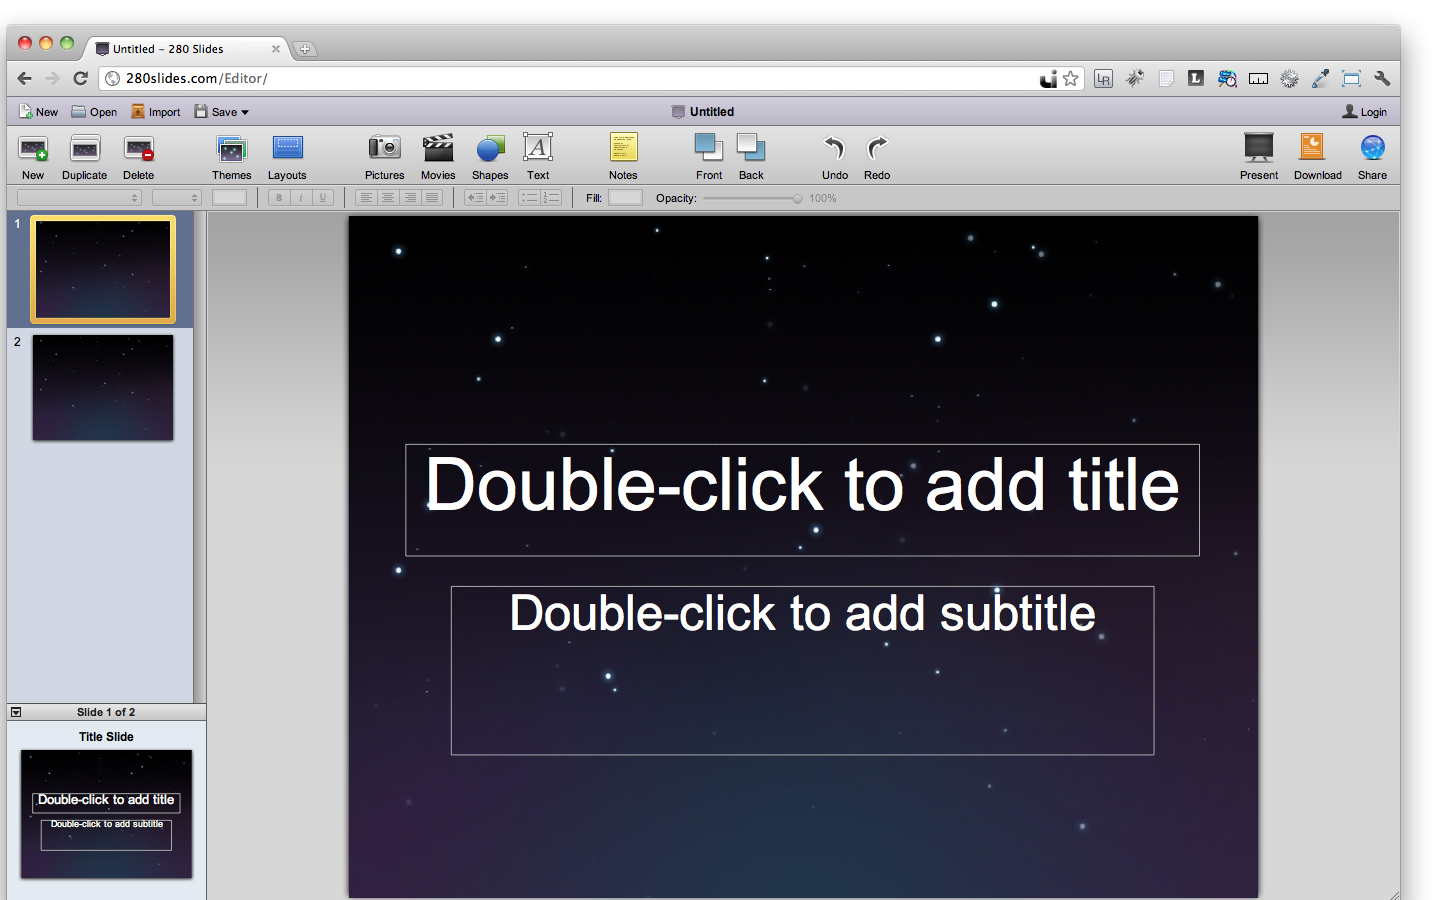
\includegraphics[width=\textwidth]{images/cappuccino_example_app.png}
\caption{Un esempio di applicazione web realizzata con Cappuccino}
\label{default}
\end{center}
\end{figure}

\subsection{Differenze ed analogie nell'interazione con l'utente}

Fino a pochi anni fa, l'interfaccia di un'applicazione web poteva essere considerata sotto molti aspetti più semplice rispetto a quella di un'applicazione desktop, per diverse ragioni.

Per iniziare, il modello di interazione con l'utente si rivelava completamente diverso. Un'applicazione web doveva sottostare ad una serie di sincronizzazioni temporali inevitabili, dovute al funzionamento del protocollo HTTP. Il modello base di interazione era la singola pagina, e ad ogni azione significativa dell'utente corrispondeva un tempo di attesa, poiché tramite una richiesta HTTP veniva richiesta al server una nuova pagina, che doveva essere trasmessa attraverso la rete e visualizzata nuovamente nel browser. Tipicamente l'utente si trovava a compilare un modulo, a premere sul pulsante di invio e ad attendere il caricamento della pagina successiva. Era presente quindi una certa sincronia e sequenzialità nelle possibili operazioni effettuate dall'utente. 

In questo aspetto risiedeva una forte differenza con le applicazioni tradizionali, che prevedono la possibilità di agire in contemporanea su diverse finestre e nelle quali l'aggiornamento dei dati visibili in seguito a determinate operazioni è pressoché immediato nella maggior parte delle situazioni.

Con la diffusione sempre più crescente della tecnologia Ajax però alcune delle differenze esistenti sono state parzialmente appianate. La possibilità di effettuare richieste HTTP asincrone attraverso l'oggetto XMLHttpRequest, supportato oggi in tutti i maggiori browser ha segnato un punto di rottura nello schema tipico di interazione tra la pagina web e il server, e di conseguenza tra l'utente e l'applicazione. Effettuando una richiesta Ajax, l'applicazione può infatti salvare il proprio stato in maniera permanente tramite uno script eseguito sul server senza che sia necessario un aggiornamento dell'intera pagina, in un processo totalmente trasparente per l'utente. Allo stesso modo, tramite Javascript è possibile aggiornare alcune aree della pagina con i dati ricevuti dal server, senza effettuare una nuova richiesta HTTP sincrona.

\begin{figure}[htbp]
\begin{center}
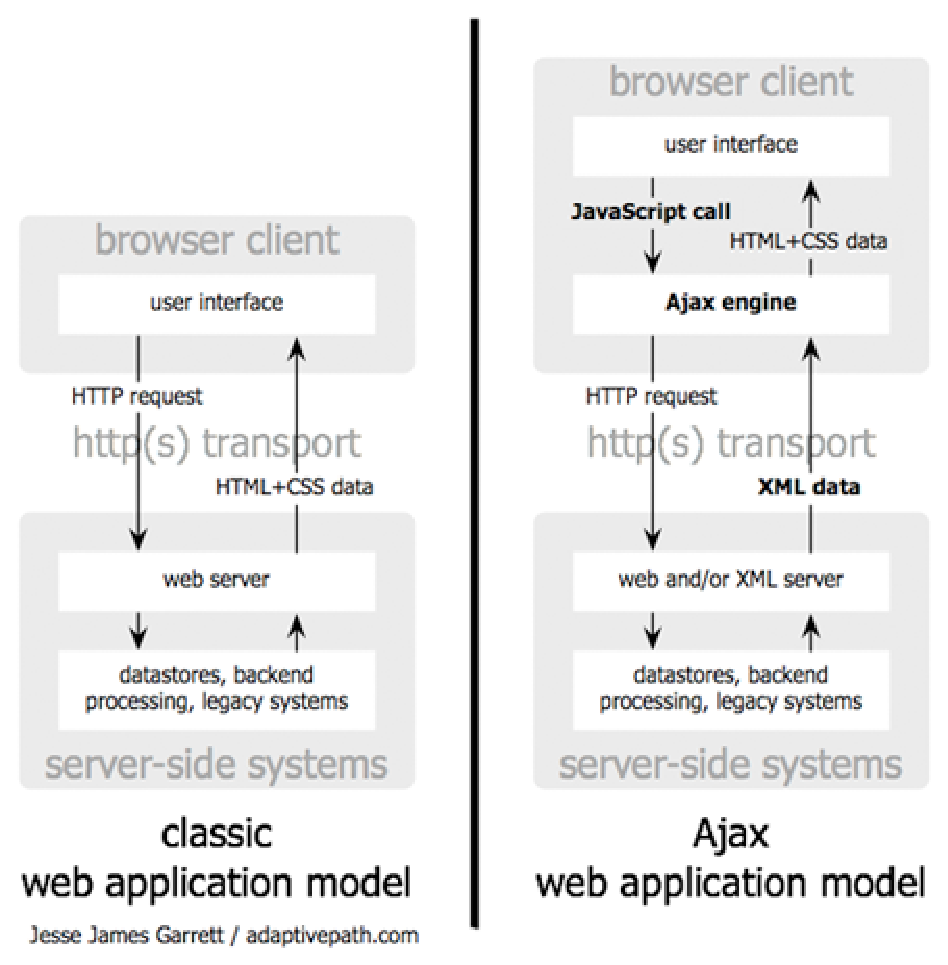
\includegraphics[scale=0.8]{images/classic_vs_ajax.eps}
\caption{Il modello di un'applicazione web tradizionale (a sinistra) a confronto con quello di un'applicazione che utilizza richieste asincrone (a destra), secondo \cite{ajaxGarrett} }
\label{default}
\end{center}
\end{figure}

Le applicazioni che fanno uso di questo nuovo paradigma rimangono comunque legate alle tecnologie tradizionali, come HTML, CSS e Javascript (\cite{ajaxGarrett}). Pertanto queste nuove tendenze vanno sicuramente esplorate anche nell'ambito dei test, ma costituiscono un elemento di aggiunta e non di stravolgimento rispetto alle tecniche già consolidate.

 

